\documentclass[12pt,twoside]{article}

\usepackage[backend=biber,style=alphabetic]{biblatex} 
\addbibresource{ref.bib}  


%%%%%%%%%%%%%%%%%%%%%%%%%%%%%%%%%%%%%%%%%%%%%%%%%%%%%%%%%%%%%%%%%%%%%%%%%%%%%

% Definitions for the title page
% Edit these to provide the correct information
% e.g. \newcommand{\reportauthor}{Timothy Kimber}

\newcommand{\reporttitle}{A digital interface designed for sharing diagnostic medical imaging with patients}
\newcommand{\reportauthor}{Laura Hagege LH}
\newcommand{\supervisor}{Fernando Bello}
\newcommand{\degreetype}{Msc. Computing Science}

%%%%%%%%%%%%%%%%%%%%%%%%%%%%%%%%%%%%%%%%%%%%%%%%%%%%%%%%%%%%%%%%%%%%%%%%%%%%%

% load some definitions and default packages
%%%%%%%%%%%%%%%%%%%%%%%%%%%%%%%%%%%%%%%%%
% University Assignment Title Page 
% LaTeX Template
% Version 1.0 (27/12/12)
%
% This template has been downloaded from:
% http://www.LaTeXTemplates.com
%
% Original author:
% WikiBooks (http://en.wikibooks.org/wiki/LaTeX/Title_Creation)
%
% License:
% CC BY-NC-SA 3.0 (http://creativecommons.org/licenses/by-nc-sa/3.0/)
% 
%
%%%%%%%%%%%%%%%%%%%%%%%%%%%%%%%%%%%%%%%%%
%----------------------------------------------------------------------------------------
%	PACKAGES AND OTHER DOCUMENT CONFIGURATIONS
%----------------------------------------------------------------------------------------
\usepackage[a4paper,hmargin=2.8cm,vmargin=2.0cm,includeheadfoot]{geometry}
\usepackage{textpos}
\usepackage{natbib} % for bibliography
\usepackage{tabularx,longtable,multirow,subfigure,caption}%hangcaption
\usepackage{fncylab} %formatting of labels
\usepackage{fancyhdr} % page layout
\usepackage{url} % URLs
\usepackage[english]{babel}
\usepackage{amsmath}
\usepackage{graphicx}
\usepackage{dsfont}
\usepackage{epstopdf} % automatically replace .eps with .pdf in graphics
\usepackage{backref} % needed for citations
\usepackage{array}
\usepackage{latexsym}
\usepackage[pdftex,pagebackref,hypertexnames=false,colorlinks]{hyperref} % provide links in pdf

\hypersetup{pdftitle={},
  pdfsubject={}, 
  pdfauthor={},
  pdfkeywords={}, 
  pdfstartview=FitH,
  pdfpagemode={UseOutlines},% None, FullScreen, UseOutlines
  bookmarksnumbered=true, bookmarksopen=true, colorlinks,
    citecolor=black,%
    filecolor=black,%
    linkcolor=black,%
    urlcolor=black}

\usepackage[all]{hypcap}


%\usepackage{color}
%\usepackage[tight,ugly]{units}
%\usepackage{float}
%\usepackage{tcolorbox}
%\usepackage[colorinlistoftodos]{todonotes}
% \usepackage{ntheorem}
% \theoremstyle{break}
% \newtheorem{lemma}{Lemma}
% \newtheorem{theorem}{Theorem}
% \newtheorem{remark}{Remark}
% \newtheorem{definition}{Definition}
% \newtheorem{proof}{Proof}


%%% Default fonts
\renewcommand*{\rmdefault}{bch}
\renewcommand*{\ttdefault}{cmtt}



%%% Default settings (page layout)
\setlength{\parindent}{0em}  % indentation of paragraph

\setlength{\headheight}{14.5pt}
\pagestyle{fancy}
\renewcommand{\chaptermark}[1]{\markboth{\chaptername\ \thechapter.\ #1}{}} 

\fancyfoot[ER,OL]{\sffamily\textbf{\thepage}}%Page no. in the left on odd pages and on right on even pages
\fancyfoot[OC,EC]{\sffamily }
\renewcommand{\headrulewidth}{0.1pt}
\renewcommand{\footrulewidth}{0.1pt}
\captionsetup{margin=10pt,font=small,labelfont=bf}


%--- chapter heading

\def\@makechapterhead#1{%
  \vspace*{10\p@}%
  {\parindent \z@ \raggedright \sffamily
    \interlinepenalty\@M
    \Huge\bfseries \thechapter \space\space #1\par\nobreak
    \vskip 30\p@
  }}

%---chapter heading for \chapter*  
\def\@makeschapterhead#1{%
  \vspace*{10\p@}%
  {\parindent \z@ \raggedright
    \sffamily
    \interlinepenalty\@M
    \Huge \bfseries  #1\par\nobreak
    \vskip 30\p@
  }}

\allowdisplaybreaks

% load some macros
% Here, you can define your own macros. Some examples are given below.

\newcommand{\R}[0]{\mathds{R}} % real numbers
\newcommand{\Z}[0]{\mathds{Z}} % integers
\newcommand{\N}[0]{\mathds{N}} % natural numbers
\newcommand{\C}[0]{\mathds{C}} % complex numbers
\renewcommand{\vec}[1]{{\boldsymbol{{#1}}}} % vector
\newcommand{\mat}[1]{{\boldsymbol{{#1}}}} % matrix


\date{September 2018}

\begin{document}

% load title page
% Last modification: 2015-08-17 (Marc Deisenroth)
\begin{titlepage}

\newcommand{\HRule}{\rule{\linewidth}{0.5mm}} % Defines a new command for the horizontal lines, change thickness here


%----------------------------------------------------------------------------------------
%	LOGO SECTION
%----------------------------------------------------------------------------------------


\includegraphics[width = 4cm]{./figures/imperial}\\[0.5cm] 

\center % Center remainder of the page

%----------------------------------------------------------------------------------------
%	HEADING SECTIONS
%----------------------------------------------------------------------------------------

\textsc{\Large Imperial College London}\\[0.5cm] 
\textsc{\large Department of Computing}\\[0.5cm] 

%----------------------------------------------------------------------------------------
%	TITLE SECTION
%----------------------------------------------------------------------------------------

\HRule \\[0.4cm]
{ \huge \bfseries \reporttitle}\\ % Title of your document
\HRule \\[1.0cm]

%----------------------------------------------------------------------------------------
%	SUB TITLE SECTION
%----------------------------------------------------------------------------------------

\textsc{\large --- Background and Progress Report ---}\\[0.5cm] 
 
%----------------------------------------------------------------------------------------
%	AUTHOR SECTION
%----------------------------------------------------------------------------------------



\emph{by} \\
\reportauthor % Your name

~

\emph{Supervisor:} 
\supervisor % Supervisor's Name




%----------------------------------------------------------------------------------------
%	FOOTER & DATE SECTION
%----------------------------------------------------------------------------------------
\vfill % Fill the rest of the page with whitespace
Submitted in partial fulfillment of the requirements for the MSc degree in
\degreetype~of Imperial College London\\[0.5cm]

\makeatletter
\@date 
\makeatother


\end{titlepage}



% page numbering etc.
%\pagenumbering{roman}
%\clearpage{\pagestyle{empty}\cleardoublepage}
%\setcounter{page}{1}
%\pagestyle{fancy}

%%%%%%%%%%%%%%%%%%%%%%%%%%%%%%%%%%%%
%\begin{abstract}
%Your abstract.
%\end{abstract}

%\cleardoublepage
%%%%%%%%%%%%%%%%%%%%%%%%%%%%%%%%%%%%
%\section*{Acknowledgments}
%Comment this out if not needed.

\clearpage{\pagestyle{empty}\cleardoublepage}

%%%%%%%%%%%%%%%%%%%%%%%%%%%%%%%%%%%%
\begin{abstract}
\normalsize



"The abstract is a very brief summary of the report's contents. It should be about half page long. Somebody unfamiliar with your project should have a good idea of what it is about having read the abstract alone and will know whether it will be of interest to them."

\end{abstract}
\cleardoublepage


%%%%%%%%%%%%%%%%%%%%%%%%%%%%%%%%%%%%
\renewcommand{\abstractname}{Acknowledgements}
\begin{abstract}

"It is usual to thank those individuals who have provided particularly useful assistance, technical or otherwise, during your project. Your supervisor will obviously be pleased to be acknowledged as they will have invested quite a lot of time overseeing your progress."

Person to thank:
\newline \vspace{5mm}
- I would like to express my deep gratitude to Professor Dr Fernando Bello
\newline \vspace{5mm}
- Will Cox
\newline \vspace{5mm}
- Co-workers at Chelsea and westminster hospital
\newline \vspace{5mm}
- Developper community over the internet and around me 
\newline \vspace{5mm}



\end{abstract}
\cleardoublepage


%%%%%%%%%%%%%%%%%%%%%%%%%%%%%%%%%%%%
%--- table of contents
%\fancyhead[RE,LO]{\sffamily {Table of Contents}}
\tableofcontents 

\clearpage{\pagestyle{empty}\cleardoublepage}
\pagenumbering{arabic}
\setcounter{page}{1}
\fancyhead[LE,RO]{\slshape \rightmark}
\fancyhead[LO,RE]{\slshape \leftmark}


%%%%%%%%%%%%%%%%%%%%%%%%%%%%%%%%%%%%
\section{Introduction}

According to a study published in January 2018 from \textbf{National Health Service (NHS) England} [2], 41.4 million \textbf{imaging tests} have been reported in England between October 2016 and December 2017. Indeed, \textbf{medical imaging} exams are routinely used all over the world to explore internal body structures and/or diagnose diseases. This generic term encompasses various clinical imaging techniques, such as, \textbf{Magnetic Resonance Imaging} (MRI), \textbf{Computerized Tomography} (CT-Scan) or \textbf{X-Ray}, which produce a 2D or 3D representation of physical internal structures. 

\newline \vspace{5mm}

Methods used for those exams are common, and since the introduction of the \textbf{DICOM standard} in 1985 [3], so is the professional storage and communication system. However, when it comes to sharing diagnoses with patient, each country has developed its own methods. In the \textbf{United Kingdom}, it is uncommon that a patient gets, or even requests, access to its medical data. On demand, and providing payment, one can get his data, but, generally, patients have only access to their clinical report, by means of a general practitioner, and the medical images, themselves are never seen by the patient. 

\newline \vspace{5mm}

Simultaneously, with the evolution of technology continually improving access to data; access to \textbf{medical information}, including imaging data, has become more commonplace . However, the issue about sharing those sensitive data, is not only to promote access, but essentially to make those images understandable for non clinicians. Research has already been undertaken in the United States concerning the creation of a \textbf{``patient portal"} [4] - fully designed to facilitate \textbf{patient understanding} - exploring the related opportunities, and scaling different levels of benefit. 

\newline \vspace{5mm}

Considering those facts, \textbf{Dr Fernando Bello} and \textbf{Pr William Cox} have decided to deepen the subject of designing a \textbf{patient portal}. First, by exploring the \textbf{benefits and risks} of sharing medical information with patients, and thereafter by effectively building such an interface. Consequently, after a year of background researches, they offered to work on the creation of \textbf{``A digital interface designed for sharing diagnostic medical imaging with patients"}, as a final personal project to the \textbf{department of Computing Science at Imperial College of London}, together with the \textbf{Chelsea and Westminster Hospital}. Aiming to build an interface \textbf{suitably made for imaging patients} in order to let them access and understand their medical results in the most significant and comprehensible way.

\newline \vspace{5mm}
The following report contains an overview of the work undertaken during almost three month beginning mid May 2018 under the supervision of \textbf{Dr Fernando Bello} and \textbf{Pr William Cox}. The following sections will develop in a logical order - for better understanding - the several steps reached during the conception of the interface, including issues, skills earned and personal review. 

\newline \vspace{5mm}
//Introduce the plan - will do once it is certain

  


 







\clearpage



%%%%%%%%%%%%%%%%%%%%%%%%%%%%%%%%%%%%
\section{Background and Related Work}
\subsection{Project context}
%will work and goal
--> Will PhD work 
\newline
--> litterature review
\newline
--> developp section about benefit



Providing medical data to a patient is always a delicate step in a medical procedure. According to medical imaging, there are 2 manners to share data with patient, either under the control of a clinical expert, or recently via standalone technologies which could left the patient with some doubts.  

While sharing this data on a digital interface > benefit tot. discuss
Subject of will pHD, define in its report + litterature review, a lot of article 

Before beginig to work --> read though those paper and understand the challenges of this project and why 


Challenges to create an interface that could be sufficiant or provide enough to guide on the right track



PATIENT PORTAL = view medical report online 
PORTAL CAN BE "DYNAMIC AND TAILORED to patient information preference"  IPAD 2

creating an interface that can be progressively adapted in order to fit patient needs.

Why the project: 

Medical Imaging exams are routinely used to explore the human body and detect disease. 

In the litterature: experience and perceive patient needs in terms of information sharing 
--> IPAD2 = making a study on the benefit of sharing information with patient, how to share, what to share, how will patients reacts - focusedd on lung cancer patient (Los angeles)

A LOOOOOt of litterature in this field, a lot of background work on the benefit, my work come as the final stage of this question

2 BENEFIT: related and unrelated (education etc)

WILL PHD --> explore/ quantify the benefit --> MY WORK: SET UP his work in order to test it 

Some sample patient portal already done 

There are plenty of interface to deal with medical imaging but they are all made for doctors. 


With this project we want to make something accessible for the patient and valuable for them --> will levels of benefit 


With concern to provide patient with some "right" information and don't let them look over the internet for wrong answers
-> examples and talking with doctors



\clearpage
\subsection{Related Work}
Before we started to actually discuss the project goal, Will provided me with several documents, either literature reviews or articles already referenced above, concerning works and researches directly related to the project. Among those, he also provided me with the late stage report of his PhD, containing the state of play of his work at that stage. Those papers have allowed me to understand the background of the project and to identify the related issues and challenges. 

\newline \vspace{5mm}
The goal of Will's PhD is to identify the \textbf{risks and benefits} related to the creation of a patient-oriented interface. To be more precise I would cite directly from this report:

\newline \vspace{5mm}

\textit{``Intuitively, there are benefits available from sharing images with patients. Indeed, there is a wealth of research available which assesses how visualisation aids increased understanding, or promotes communication. However, little research assesses the value of radiological images in this context. Moreover, no work assesses the risks associated with sharing patients’ images with them. This is the gap which this PhD will address. The research questions for this PhD are, therefore:
\begin{itemize}
	\item Is there additional benefit that can be extracted from diagnostic images?
	\item If so, what are the requirements to enable the realisation of this benefit?"
\end{itemize}}

\newline \vspace{5mm}
Specifically, to lead his researche, he has divided benefits in two categories:
\textit{
\begin{itemize}
	\item ``Primary benefits – benefits related to the rationale for acquiring the image, e.g. diagnosis, assessment, interventional guidance
	\item Secondary benefits – benefits unrelated to the rationale for acquiring the image, e.g. education, communication, empowerment"
\end{itemize}
}

\newline \vspace{5mm}
At the moment, Will has achieved a significant work, he has completed a literature review, to set up the background and understand the issues related to the creation of a patient portal. Precisely, the aim was ``to ensure that this was a suitable subject for research and to identify any pertinent gaps in the existing knowledge.".  He also carried out a survey, questioning medical experts, supplemented with 8 semi-structured interviews in order identify and scale the related risks and benefits from a clinician point of view. the results of those works are available for consultation on \textbf{\textit{Appendix 1}. In the future the objective is to interview patients, on the same model as clinicians, to evaluate the non-clinician opinion.
  













\clearpage
\subsection{Goal definition}
Once familiar with the project background, it has been easier for me to understand the main \textbf{issues and challenges} and to have a precise idea of the goal to achieve. The objective of this project is not to simply copy and create another standard DICOM viewer but to create an interface that can be \textbf{progressively adapted to fit patient needs}. Challenges consist in buildging an interface that could be sufficient and valuable, meaning it could provide enough information to guide the patient on the right track without any simultaneous external contribution. Moreover, designing this interface should allow to identify the benefit to be realised through providing people with their imaging data, whilst also minimising the identified risks of this process.

\newline \vspace{5mm}
It has been agreed that we would together with Fernando and William, define project specifications (in terms of design and content) and that all information relative to benefits and content would be discussed mainly with William. They, also advised me to install some already existing DICOM viewer made for clinicians. They wanted me to get an idea of the kind of interface that I could produce, while keeping in mind that the goal is not to create a copy of those readers, but to produce my own patient-oriented interface.

\newline \vspace{5mm}
In the following part, I will develop the project specifications that have been produced in the early stage of the project, following multiple discussion with my tutors. Moreover, considering that I have been given complete freedom in the choice of the tools and languages to use for building the interface, I will explain the choices I have made before starting to implement my project.






\clearpage
%%%%%%%%%%%%%%%%%%%%%%%%%%%%%%%%%%%%
\section{Define Specifications and Implementation Methods}
\subsection{Early specifications}
%same as in background
Based on my previous experiences concerning the development tool for a third person, it was really important to me to define clearly the specification and limit of the project before starting to properly developp/ code it. This was on one hand to be sure to produce an interface that will suit my supervisors needs and on the other hand to avoid time waste in the future. Specifications concerning the graphical interface have been divided in five part: the basic requirements, the content, the design, the features and some further precisions. 

\newline \vspace{5mm}

During the early stage of the project we had several meetings with my two supervisor in order to define those specifications. These following specification are the specification we agreed at the time of writing the backgound and progress report.

\newline \vspace{5mm}


\begin{itemize}	
\item \textbf{Interface content:}
\newline \vspace{5mm}

\begin{itemize}
\item The interface should display patient images - images will be provided in DICOM format, and translated so that the patient can read them.
\item The interface must contain the clinical report and the simplifie version.
\item A link to NHS website will be given, so that patient could find general informations about their condition
\item Patient could get flag informations - to be filled by doctors - while exploring the images
\item Any other relevant informations related to what the DICOM files provides could be added 
\end{itemize}

\newline \vspace{5mm}

\item \textbf{Interface functionalities:}
\newline \vspace{5mm}
The interface should provide:
\begin{itemize}
\item One doctor oriented window: so, they can fill in datas (images, report) and add flag to images at their conveniance.
\item One patient oriented window: read only data (no modification allowed) and the possibility for patient to chat with doctors.

\end{itemize}

My main concern - in the context of this project - is to focus on the patient oriented side and see how far I can lead this project. This part can be really time consuming as it might need to be oftently readapted following the needs of my tutors.

Also, William recently sent me detailed general specifications concerning the patient oriented interface content/functions - Appendix 2

\newline \vspace{5mm}

\item \textbf{Interface design:}
\newline \vspace{5mm}
\begin{itemize}
\item Imaging display will depend on the provided images (MRI, CT) but not on the part of the body. Will also gave me on demand description concerning images to be display and the way to deal with it – Appendix 2.
\item Provide a side by side – or other relevant organization – that would allow the patient to get the images and the report together in a relevant way

\end{itemize}

\newline \vspace{5mm}

\item \textbf{Further precisions:}
\newline \vspace{5mm}
\begin{itemize}
\item No access to any database will be provided for the current project (security issues) 
\item Access to the interface will be local, patient would be given (upon request) a CD with their images loaded on the interface; this won’t change patient access to datas but should make them want to access it
\item Interface should include user specification/precisions for patient 
\item Benefits/specifications will have to be defined before starting implementation
\item Interface should be “windows portable” 
\end{itemize}

\newline \vspace{5mm}

\item \textbf{Interface evaluation:}
\newline \vspace{5mm}
At some point the interface should be evaluted by a panel of patient that would be ask to use it and make feedbacks.


\end{itemize}


\newline \vspace{5mm}
Eventually, thoses specifications have evolved during the realization of the project, adjusting the task the the work already performed and the encountered issues. Moreover concerning the interface Design, Will provided me with 





\clearpage
\subsection{Choosing tools- C++ and Qt}
A lot of tools are available on the Internet to create GUI interface such as Qt, WxWidget, GTK+, FLTK, FOX and some others. I couldn't compare all of them so I have decided to focus on Qt, WxWidget GTK+.

\begin{itemize} 
\item Tools Comparison: \\
I looked accross the Internet to get some testimonies about the different tools and I tried to distinguish them following several criteria - see grid below. 
According to these criteria and considering that Qt is highly recommended for beginners, I have finally decided to use Qt for this project.

\begin{figure}[ht]
\centering
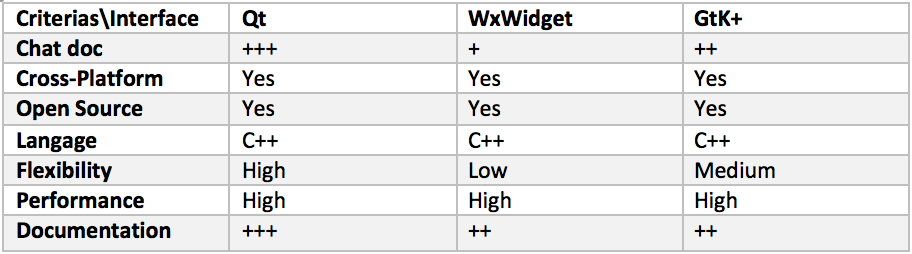
\includegraphics[width = 0.99\hsize]{./figures/comparison}
\caption{LQt, WxWidget, GTK+ comparison table}
\end{figure}
 
\item Qt familiarization: \\
In order to get used to this new tools I have decided to do Openclassroom tutorials [2].
Those tutorials have helped me to install QtCreator and to begin with some basic exercices to get familiar with Qt. I still have some tutorial to do at the current moment but I am feeling comfortable with it.


\clearpage
%%%%%%%%%%%%%%%%%%%%%%%%%%%%%%%%%%%%
\section{Understanding Imaging File Format: DICOM standard }
\subsection{Definition}
DICOM file format is a special software integrated standard format dedicated to ease data communication within different facilities in the Medical Imaging Field. This standard has been defined by the American College of Radiology (ACR) and the National Electrical Manifactural Association (NEMA) in 1983. DICOM format defines data dictionnary, data structure, file format and comes with a TCP/IP protocole to facilitate data transfer among a lot of other features. Before this standard was created it was difficult for different facilities to exchange imaging and imformation, now this format is widely use for all medical imaging areas such as CT (Computed Tomography), MRI (Magnetic Reasonance Imaging), X-Rays, Ultrasounds, etc.


\subsection{DICOM File Structure}
The \textbf{DICOM File Format} decribes how the information, encapsulated in an  \textbf{SOP instance}, should be stored in a byte stream, in a file on a physical medium. Each DICOM file is composed of two instance: a \textbf{Header} followed by a \textbf{Data Set}.

\begin{itemize} 
\item \textbf{The Header} contains 128 bytes preamble (which are all set to zero if it is not used) followed by 4 byte DICOM prefix (DICM). The header is not necessary included in the file but is useful to make access to data easier, indeed the prefix allows to quickly acknowledge DICOM format. Besides, no structure is required for the preamble.  

\item \textbf{The Data Set} is organised as consecutive \textbf{DICOM Data Element} (or Data Attribute), referenced in the DICOM standard [10]. Those Data Element can represent various information, from the patient name and birth to theimage pixels. More precisely one \textbf{DICOM Data Element} is \textit{one unit of information} corresponding to one encoded \textbf{Information Object Definition (IOD) Attribute}, defined above. Figure 4 gives a representation of the DICOM File structure.
\end{itemize}

\begin{figure}[ht]
\centering
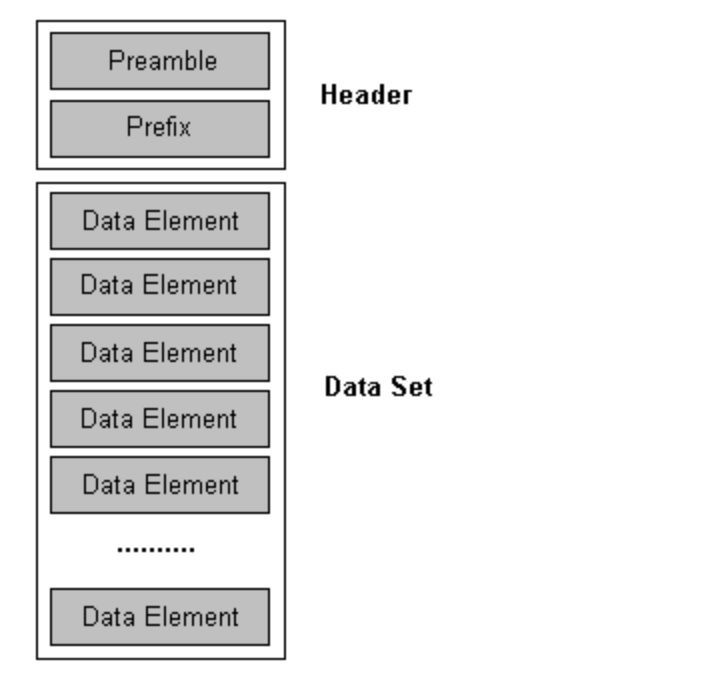
\includegraphics[width = 0.45\hsize]{./figures/DicomFileFormat}
\caption{Basic DICOM File Structure}
\end{figure}

\newline \vspace{5mm}
\textbf{DICOM Data Element} are \textit{Tag Element}, therefore DICOM can be said to be a tag file format, this mean that each element is referenced by a unique \textbf{Tag Number} defining the element and its properties. In the Data Set, Data Elements are ordered by increasing Tag Number. Each Data Element is made of the same range of consecutive fields: 
\begin{itemize} 
\item \textbf{Tag Number}: it consists in an ordered pair of 16 bits unsigned integer of the form (gggg,eeee)  representing the \textit{Group Number} - defining the Information Entity - followed by the \textit{Element Number} - defining the attribute. For example, in the tag (0028,0010), the Group Number is 0028 and correspond to the Image group, the Element Number is 0010 and correspond to the row (especially to the length of the image in pixels).
\item \textbf{Value Representation}: it defines the data type of the element. As the Tag Number already implies the data type, the value representation can be omitted.
\item \textbf{Value Length}: either 16 or 32 bits element, this defines the length of the following value.
\item \textbf{Value Field}: consists in an even number of bytes containing the value of the element; this field can contain the Value Multiplicity, which would specified the number of values that can be encoded in the field. 
\end{itemize}

\begin{figure}[ht]
\centering
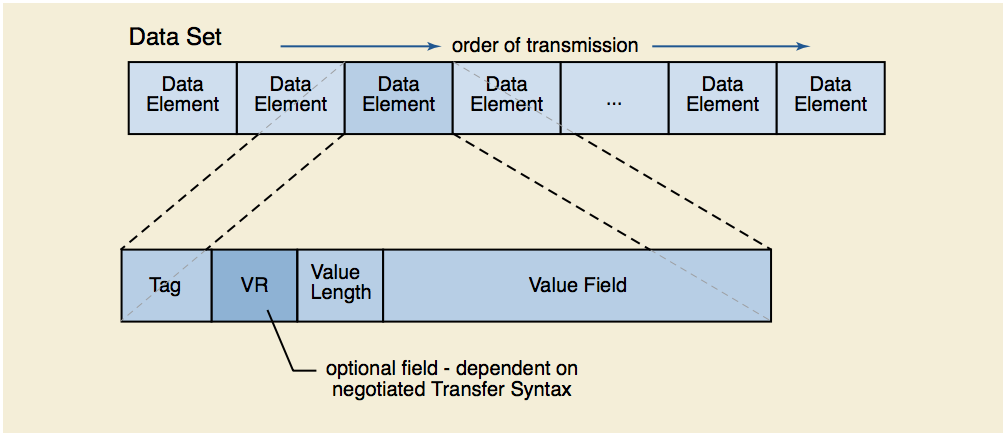
\includegraphics[width = 0.8\hsize]{./figures/DataSetandDataElement}
\caption{Data Set and Data Element structure}
\end{figure} 







\clearpage
%%%%%%%%%%%%%%%%%%%%%%%%%%%%%%%%%%%%
\section{Implementation}
\subsection{Code Structure}
\textbf{1.What is DCMTK}
\newline
DCMTK is an open-source collection of libraries and applications that has been made to  deals with the DICOM format while developping an independant application. This software is widely used by hospitals, companies or private individuals that aim at creating DICOM related desktop software. DCMTK provide several classes and script in order to treat, construct, and convert DICOM files and an internal worklist server in order store, send or receive images.

\newline
DCMTK source code repository is available on Github and free for downloading. It is available for both Windows and Unix operating systems. For the purpus
 However dcmtk toolkit doesn't came as a prebuilt library 


\clearpage
\textbf{2.DCMTK classes and DICOM Element access}


\subsection{DCMTK library and Qt}

\clearpage
\subsection{Render DICOM Images with Qt and DCMTK}
The first challenge of this project was to render a set of DICOM Images or at least one DICOM Image. 

As I already explained, in part 4.4, the DICOM folder tree structure blablabla 


However IMG0000 file are not of only one type, this file can be either:
\begin{itemize}
	\item One single frame DICOM Image
	\item Several single frame DICOM Images
	\item One multiframe DICOM Image
\end{itemize}

Objectively, single and multi frame images only differ by the size of the file.

\newline \vspace{5mm}	
\textbf{1. Display one image:}

\newline \vspace{5mm}	

The DCMTK library that I installed contains several classes that should make DICOM Images treatment easier.
The class I used to deal with DICOM Images files is called DicomImage, the class structure and related functions are available on DCMTK website [8888].
The class is provided with four different constructors and depending on the given parameters this class allows to deal with single frame and multiframe images. Information about the constructor I choosed are available on Appendix XXX figure YYY


\begin{itemize}
	\item Display single frame DICOM Image:
	
	\begin{center}
	\textit{DicomImage *DcmImg = new DicomImage(path)}
	\end{center}
	
	
	\item Display multiframe DICOM Image:
	
	\begin{center}
	\textit{DicomImage *DcmImg = new DicomImage(path,0,index,1)}
	\end{center}
	
	\textit{index} being the index of the frame to display
	
\end{itemize}

The variable \textit{path} is a string and contains the absolut path to the DICOM Image file.
\newline \vspace{5mm}


Once I got the DicomImage object, I need to get the pixels in order to have the opportunity to use QImage class thereafter. Here again DCMTK provide me with the function \textit{getOutputData()} - see Appendix XX figure ZZ -. The corresponding line of code is:
\newline \vspace{5mm} 

	\begin{center}
	\textit{uint8_t* pixelData= DcmImg->getOutputData(8)}
	\end{center}

\newline \vspace{5mm}  
Explain what is uint8_t



Finally I only need to use two classes provided by Qt to render the DICOM Image on my application:

\newline \vspace{5mm} 

	\begin{center}
	\textit{uint8_t* pixelData= DcmImg->getOutputData(8)}
	\end{center}

\newline \vspace{5mm}  

QIMage only takes pixel and a scene can only display QPixmap element see appendix


\newline \vspace{5mm}	

\textbf{2. Store and display successive images of the serie}

\newline \vspace{5mm}	







\clearpage
%%%%%%%%%%%%%%%%%%%%%%%%%%%%%%%%%%%%
\section{Design and Features}
\subsection{Design with QtDesigner}
%Should definitely takl about my issues because project not really reachable


\clearpage
\subsection{Features implementation}
\input{src/section/designfeatures/featuresdevelopment}



\clearpage
%%%%%%%%%%%%%%%%%%%%%%%%%%%%%%%%%%%%


\section{Results}
\clearpage
\subsection{Final output}
\input{src/section/results/design}

\clearpage
\subsection{Third party feedback}
\input{src/section/results/patienteval}


\clearpage
%%%%%%%%%%%%%%%%%%%%%%%%%%%%%%%%%%%%


\section{Evaluation}

\clearpage
\subsection{Personal evaluation}
--> explain some choice 
\newline
--> show calcul for different plan output

\clearpage
\subsection{Ethic and LSEPI checklist}


\clearpage
%%%%%%%%%%%%%%%%%%%%%%%%%%%%%%%%%%%%
\section{Conclusions and Future work}



\clearpage
%%%%%%%%%%%%%%%%%%%%%%%%%%%%%%%%%%%%
\section{Appendix}
\clearpage

\subsection {Appendix  - Expert Questionnaire Results from William PhD}
\begin{figure}[ht]
\centering
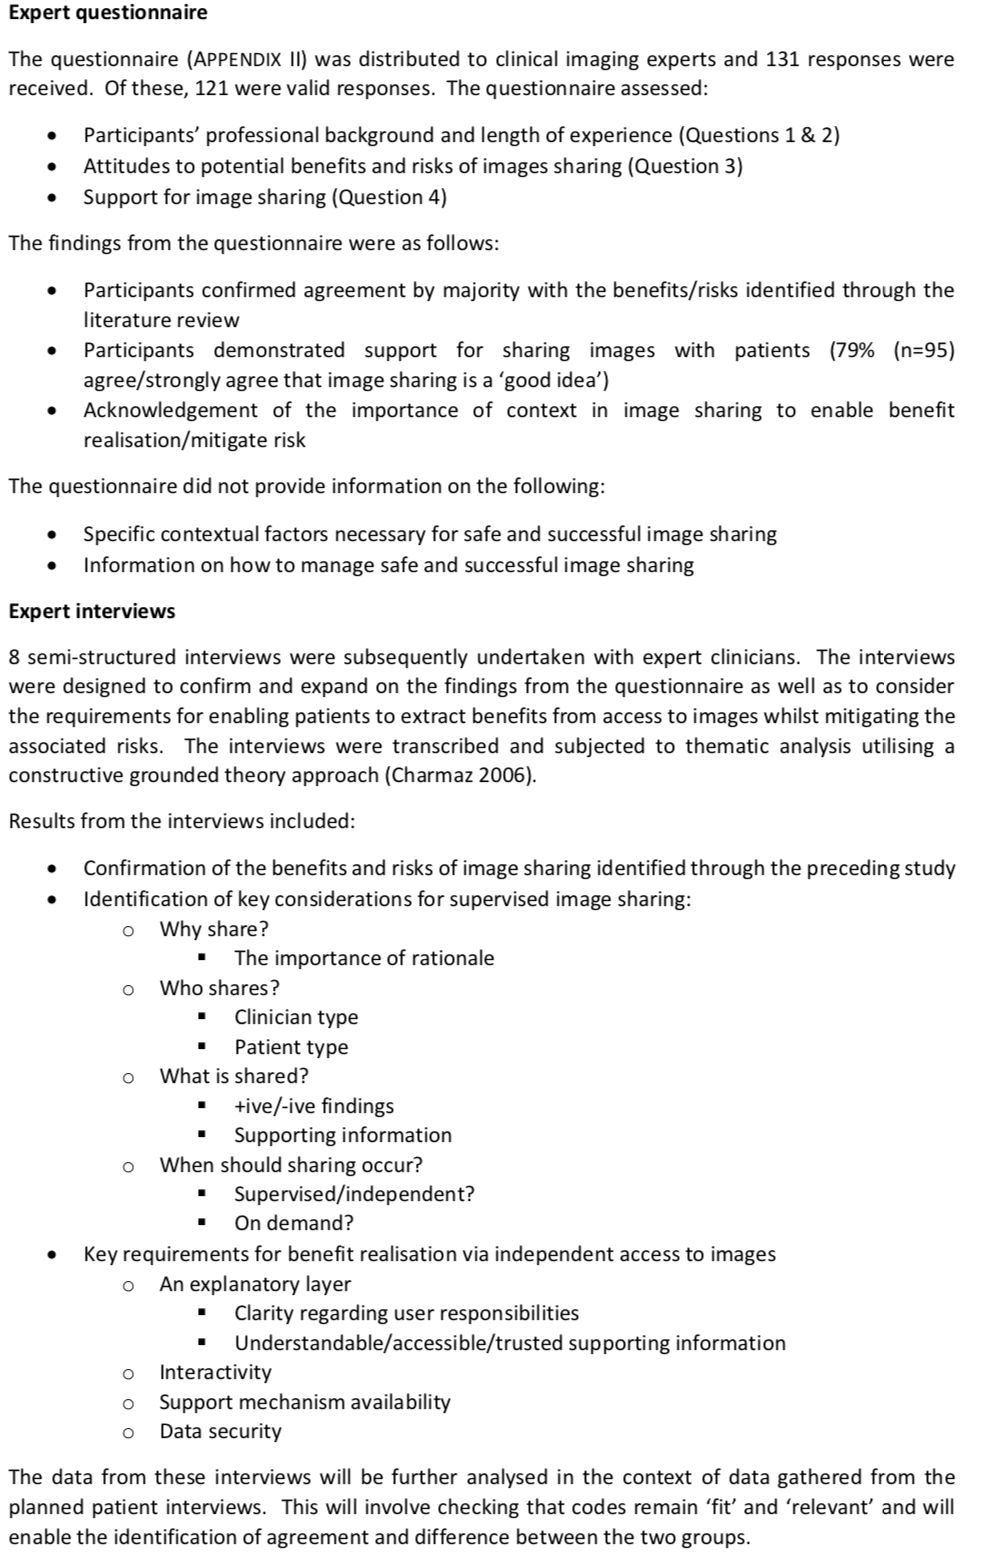
\includegraphics[width = 0.80\hsize]{./figures/ExpertResult}
\caption{Expert Questionnaire Results}
\end{figure}




\clearpage

\subsection {Appendix  - General Specification}
\begin{figure}[ht]
\centering
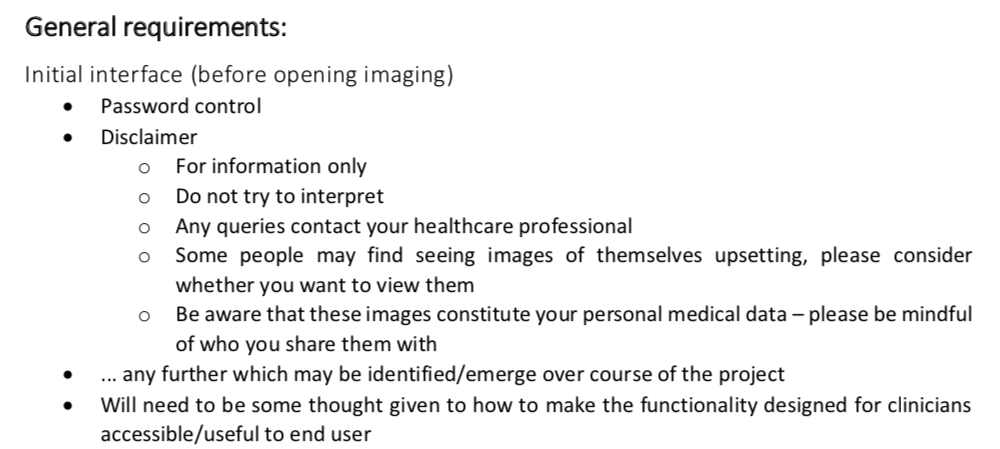
\includegraphics[width = 0.95\hsize]{./figures/GeneralSpec1}
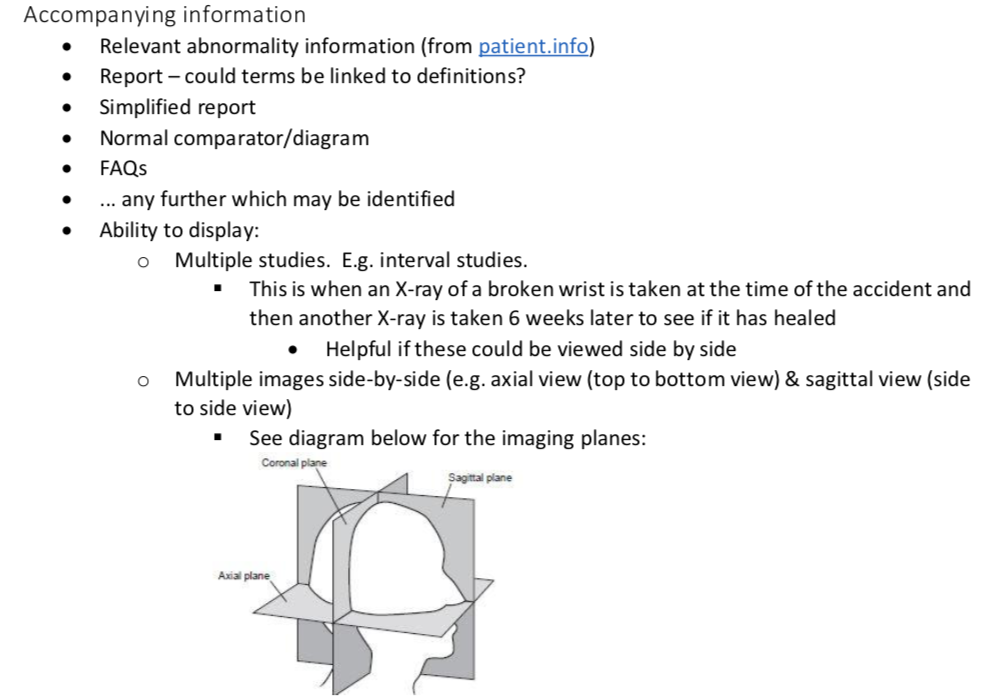
\includegraphics[width = 0.95\hsize]{./figures/GeneralSpec2}
\end{figure}



\clearpage

\begin{figure}[ht]
\centering
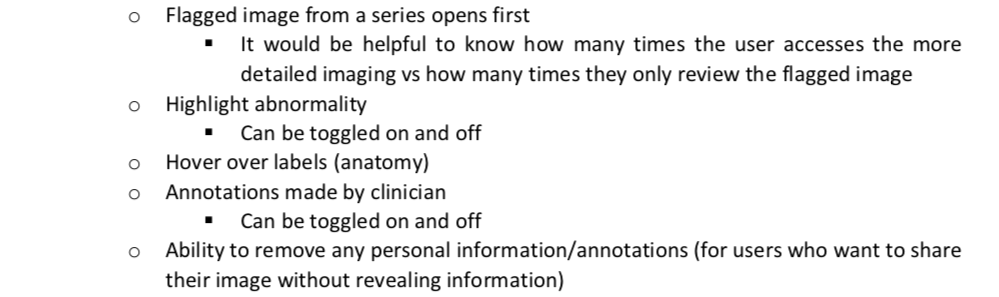
\includegraphics[width = 0.95\hsize]{./figures/GeneralSpec3}
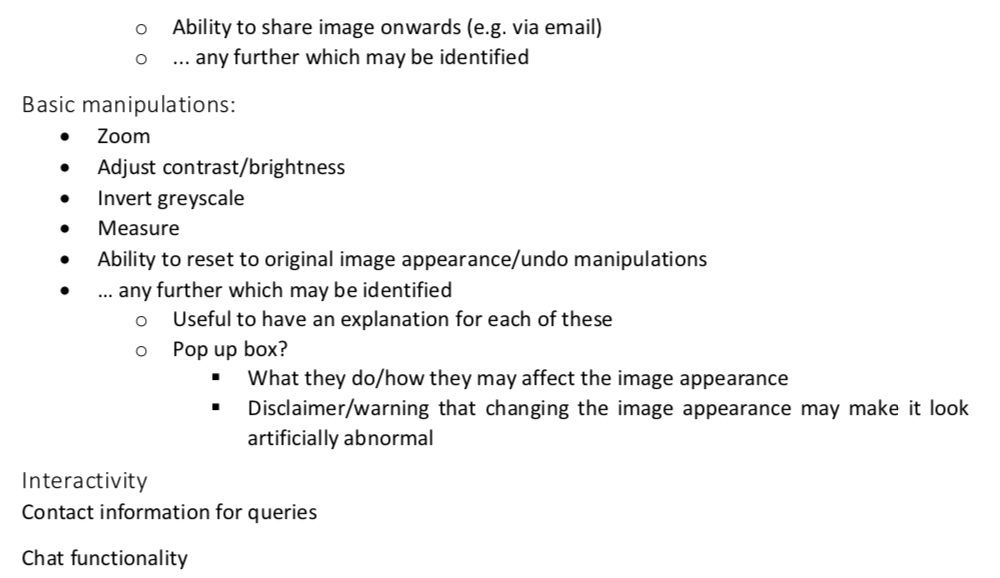
\includegraphics[width = 0.95\hsize]{./figures/GeneralSpec4}
\end{figure}

\clearpage

\subsection {Appendix  - Imaging Specification}
\begin{figure}[ht]
\centering
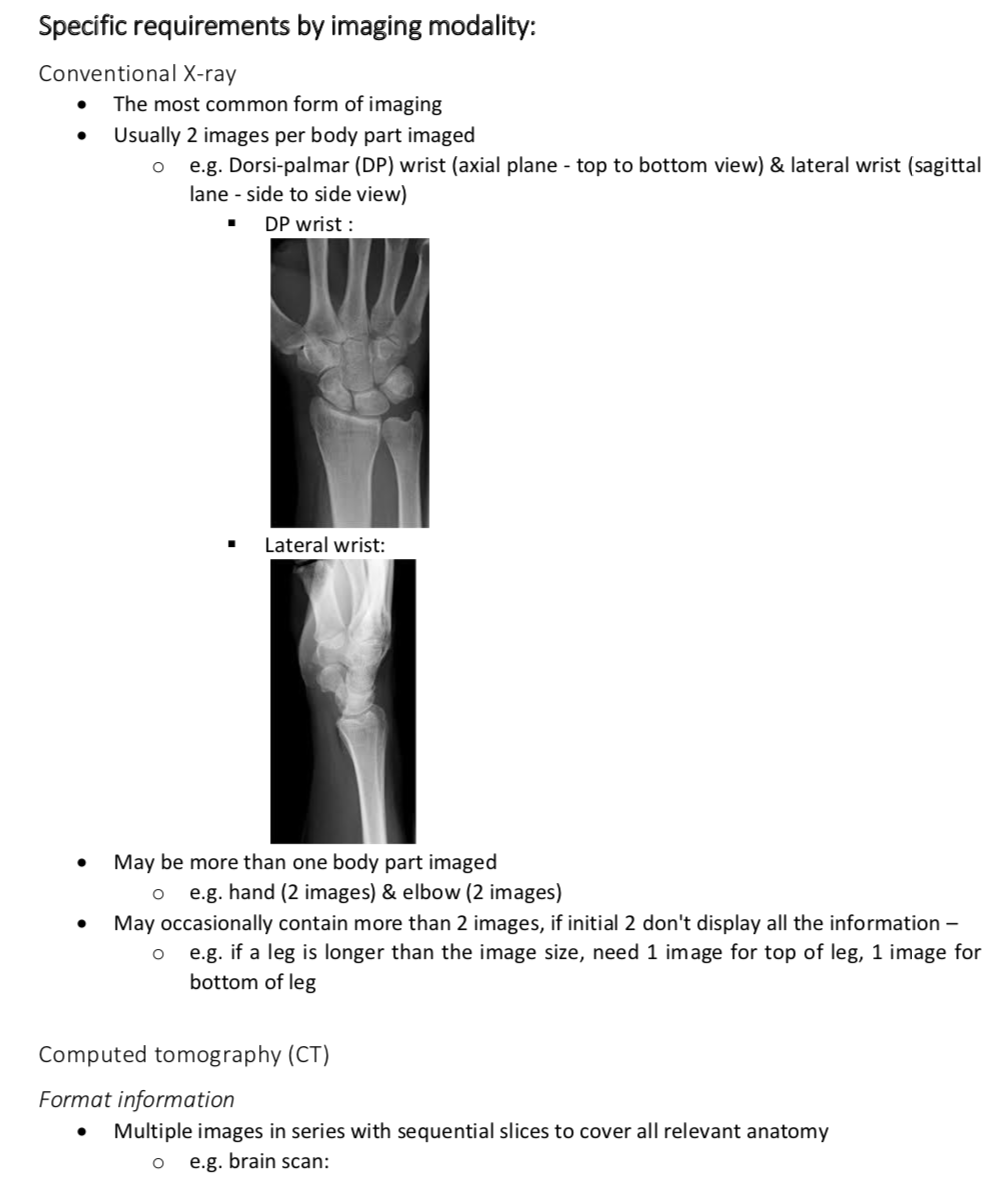
\includegraphics[width = 0.93\hsize]{./figures/ImagingSpec1}
\caption{Imaging Specification 1}
\end{figure}
\clearpage

\begin{figure}[ht]
\centering
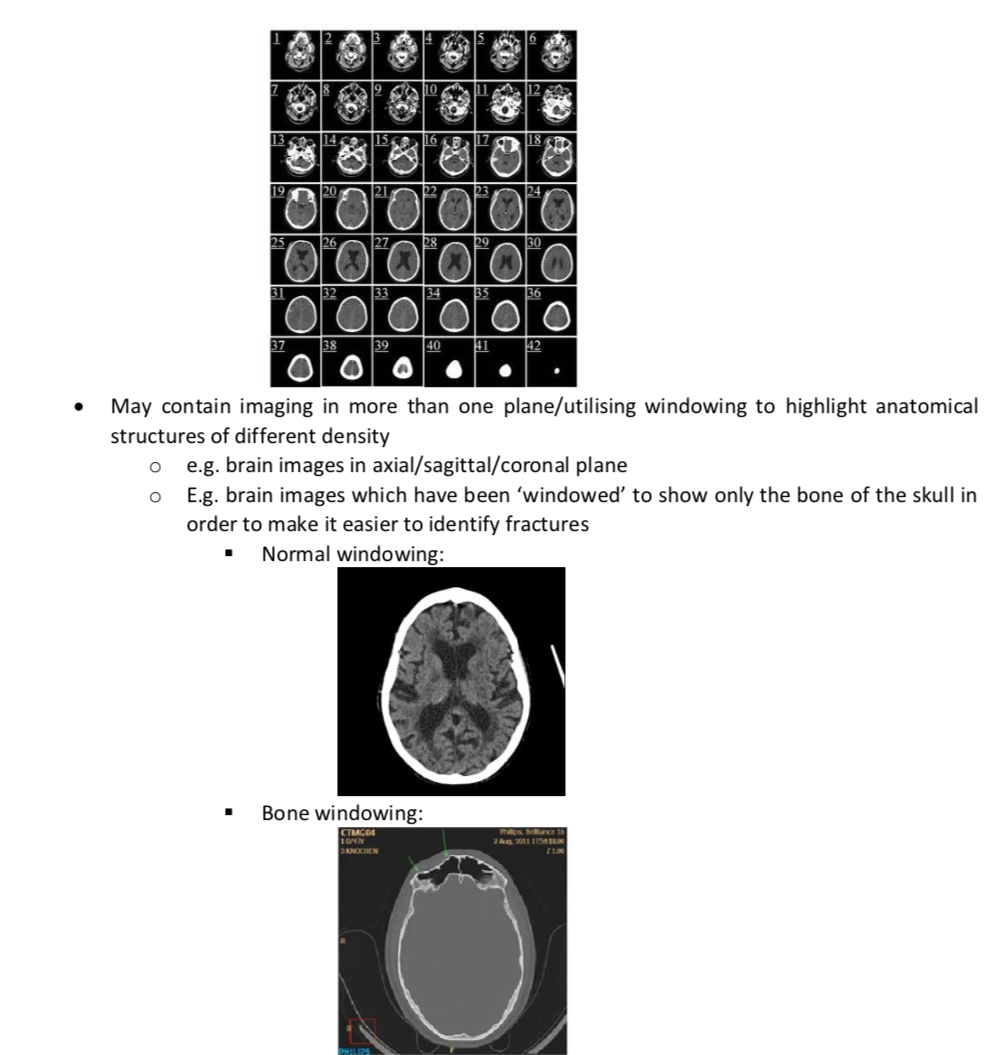
\includegraphics[width = 0.95\hsize]{./figures/ImagingSpec2}
\caption{Imaging Specification 2}
\end{figure}
\clearpage

\begin{figure}[ht]
\centering
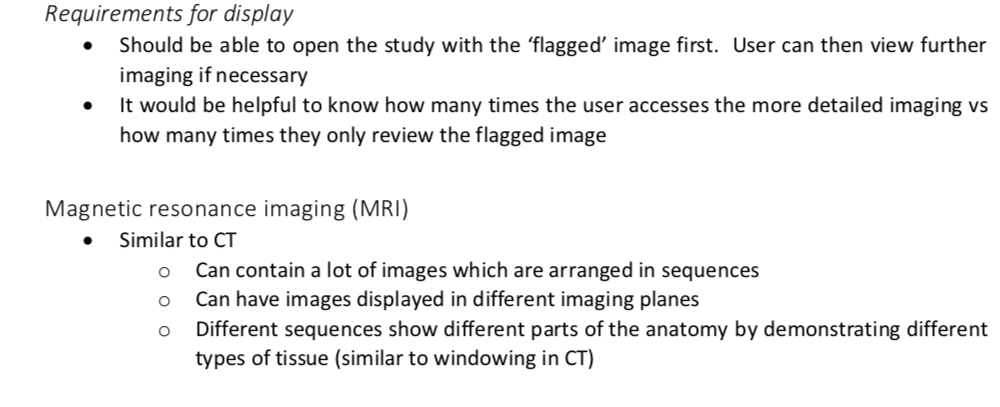
\includegraphics[width = 0.95\hsize]{./figures/ImagingSpec3}
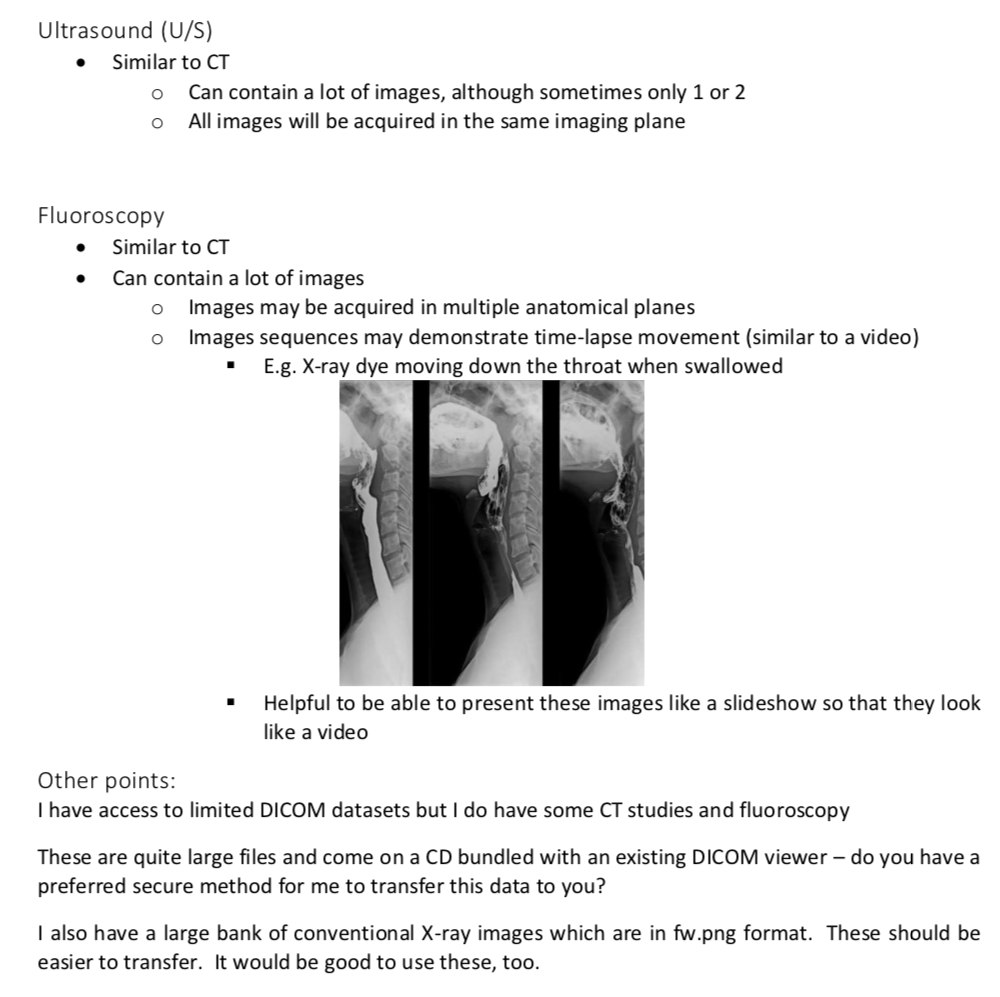
\includegraphics[width = 0.95\hsize]{./figures/ImagingSpec4}
\caption{Imaging Specification 3}
\end{figure}


\clearpage
\subsection {Appendix  - DCMTK: Relevant classes and functions declarations}
\begin{figure}[ht]
\centering
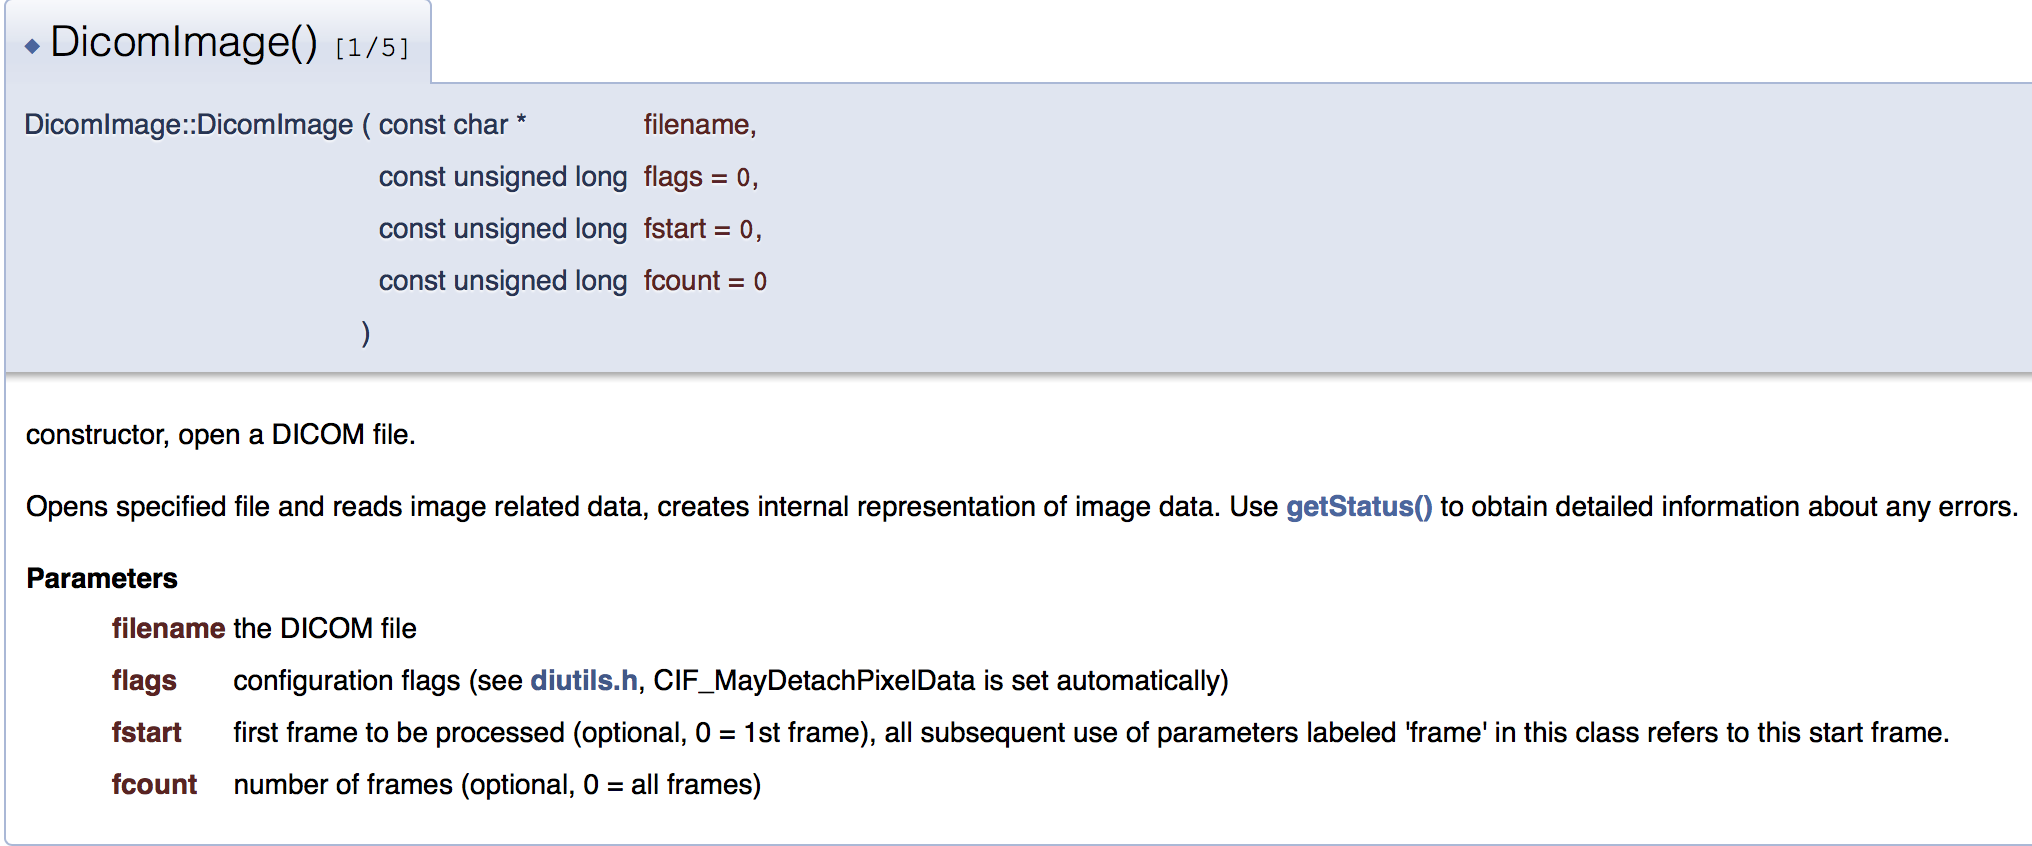
\includegraphics[width = 0.95\hsize]{./figures/DicomImageConstructor}
\caption{DicomImage Class Constructor}
\end{figure}


\begin{figure}[ht]
\centering
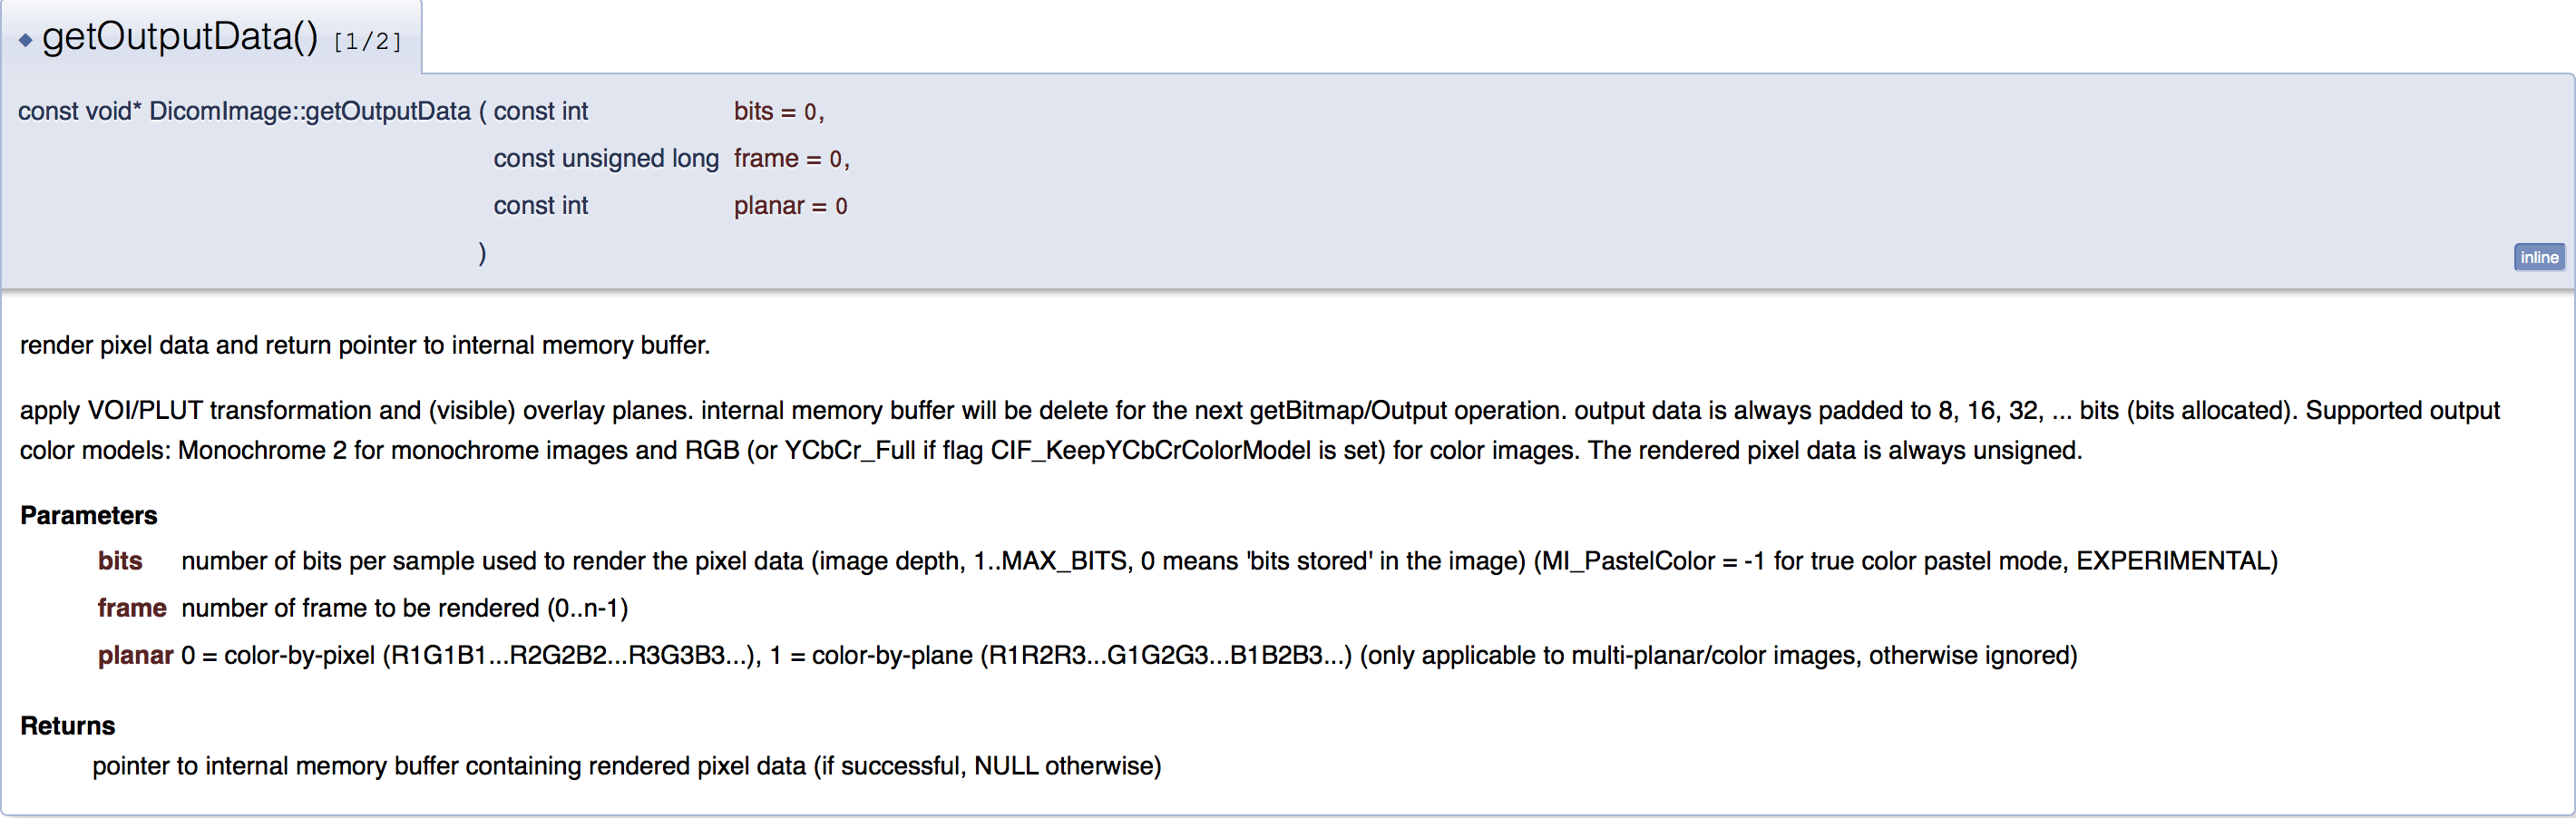
\includegraphics[width = 0.95\hsize]{./figures/getOutputData}
\caption{DicomImage getOutputData Function Definition}
\end{figure}

\clearpage
\subsection {Appendix  - Qt: Relevant classes and functions declarations}
\begin{figure}[ht]
\centering
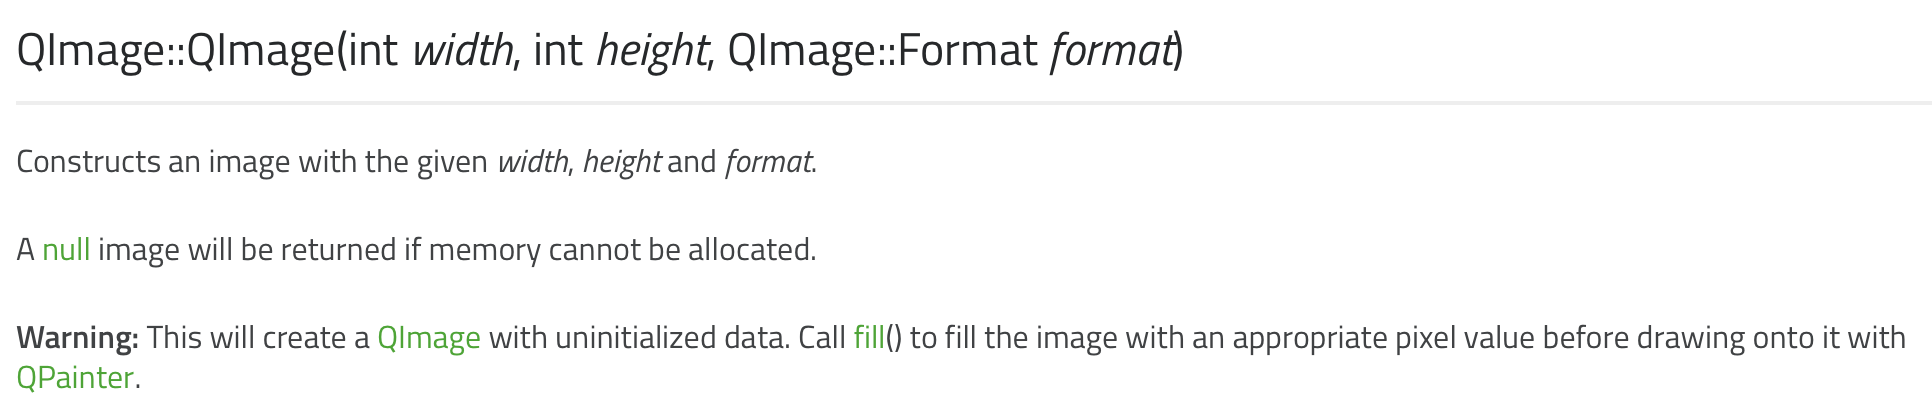
\includegraphics[width = 0.95\hsize]{./figures/QImage}
\caption{QImage contructor}
\end{figure}


\begin{figure}[ht]
\centering
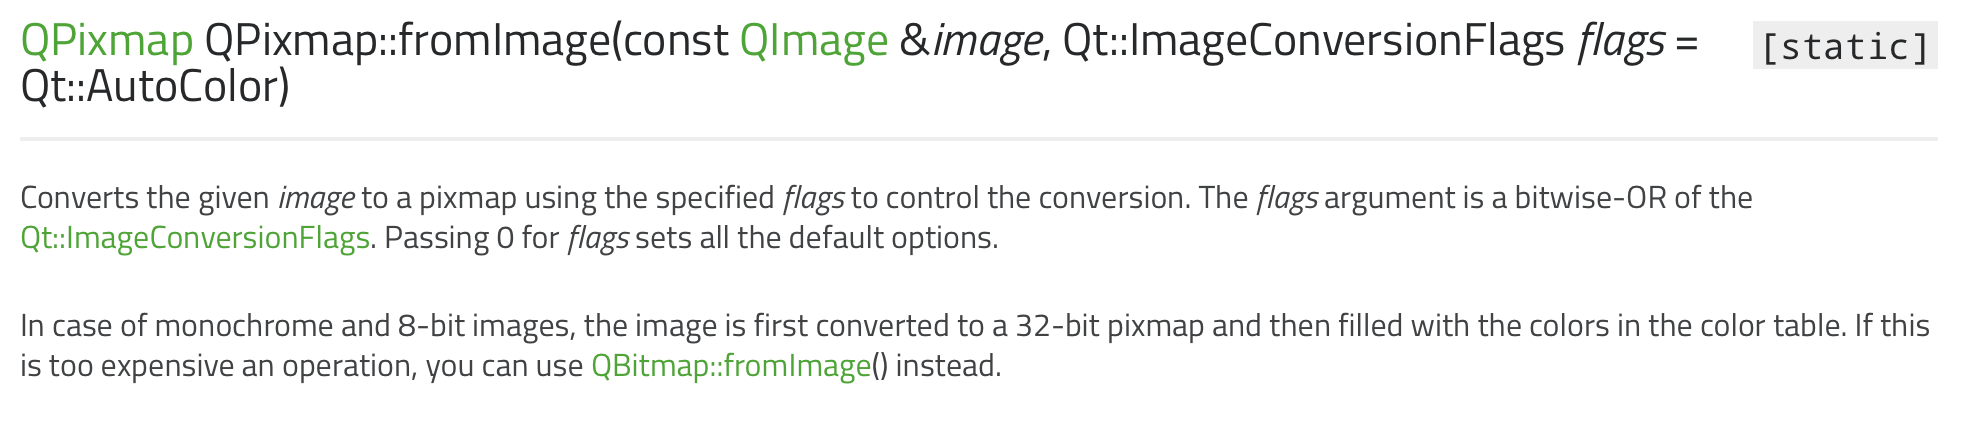
\includegraphics[width = 0.95\hsize]{./figures/QPixmap}
\caption{QPixmap static function}
\end{figure}

\clearpage
\subsection {Appendix  - Interface Design Specification}
\begin{figure}[ht]
\centering
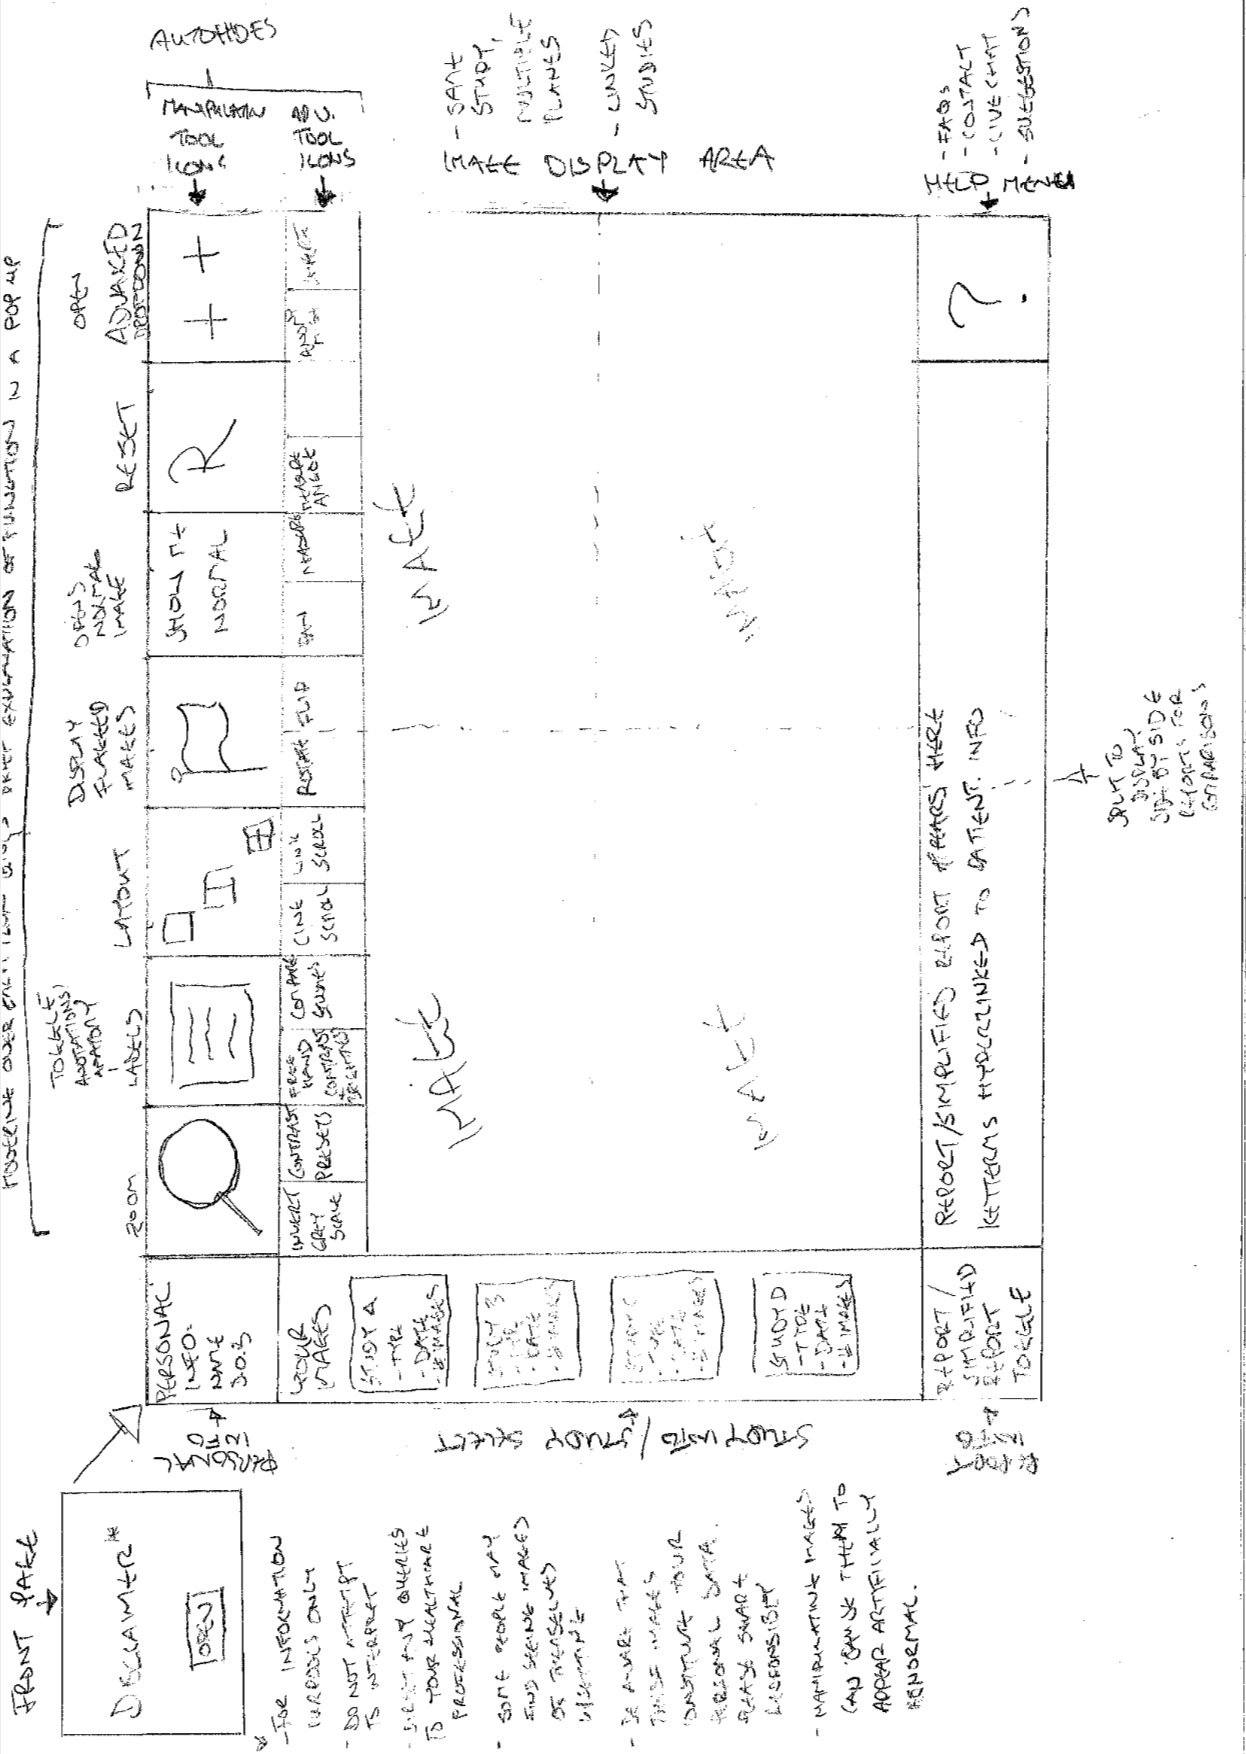
\includegraphics[width = 0.80\hsize]{./figures/InterfaceDesign}
\caption{Interface Design - Drawing Specification}
\end{figure}

\begin{figure}[ht]
\centering
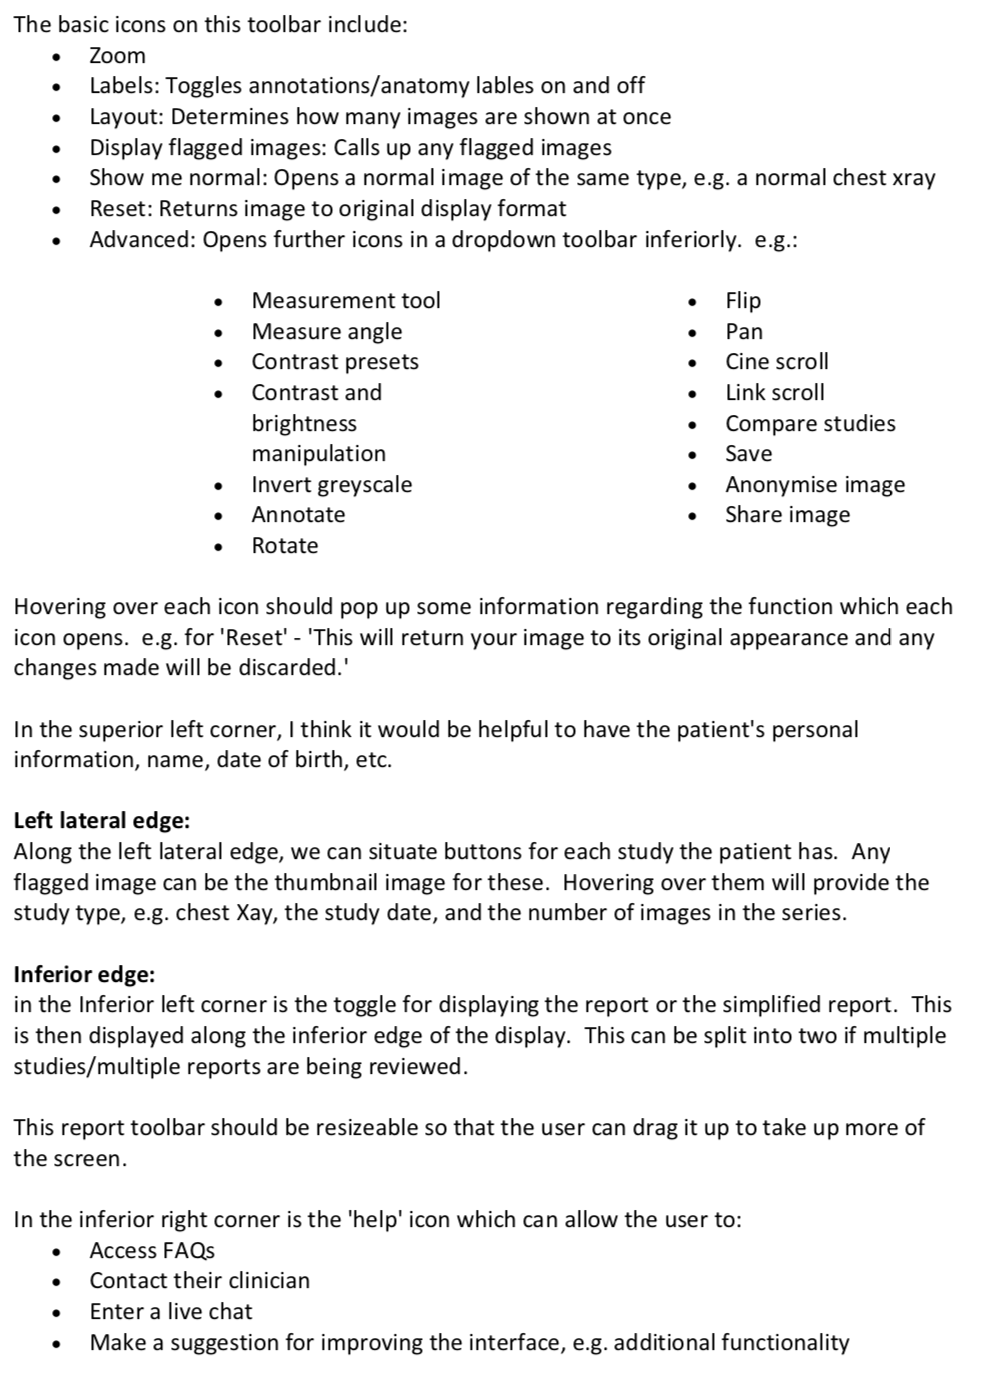
\includegraphics[width = 0.80\hsize]{./figures/DesignSpec}
\caption{Interface Design - Features Specification}
\end{figure}


%% bibliography
\printbibliography


\end{document}
